\documentclass[12pt]{article}
\usepackage[utf8]{inputenc}
\usepackage[T1]{fontenc}
\usepackage{graphicx}
\usepackage{xcolor}
\usepackage{hyperref}
\usepackage{tikz}
\usepackage{calc}
\usepackage{booktabs}
\usepackage{multicol}
%\usepackage{hyperref}

% colors
\definecolor{color1}{HTML}{00A10B}
%\definecolor{color1}{HTML}{8C260F}
\definecolor{color2}{HTML}{333333}


% fonts
\usepackage{fontspec}
\defaultfontfeatures{Mapping=tex-text}
\setmainfont
[BoldFont=Lato-Bold.ttf,
ItalicFont=Lato-Italic.ttf,
BoldItalicFont=Lato-BoldItalic.ttf]
{Lato-Regular.ttf}
\newfontfamily\headingfont[ItalicFont=Lato-BlackItalic.ttf]{Lato-Black.ttf}
%%%

\usepackage{geometry}
\geometry{a4paper,
hmargin=20mm,vmargin=20mm,
head=0ex,foot=3ex}

\linespread{1.3}

\usepackage[hang]{caption}
\DeclareCaptionFormat{upper}{#1#2\uppercase{#3}\par}
\captionsetup{labelfont={bf,color=color2},textfont={normalsize,color=color2},format = upper,figurename=FIGURE,tablename=TABLE}

%%% fancy sections
\usepackage{titlesec}
%\titleformat{\chapter}{\headingfont\LARGE\bfseries\scshape\color{color1}}{\thechapter}{1em}{}[\titlerule]
\titleformat{\section}{\color{color1}\headingfont\Large\bfseries\uppercase}{\thesection}{1em}{}[\titlerule]
\titleformat{\subsection}{\color{color1}\headingfont\large\bfseries\uppercase}{\thesubsection}{1em}{}
\titleformat{\subsubsection}{\color{color1}\headingfont\bfseries\uppercase}{\thesubsubsection}{1em}{}
%%%

% head and foot
\usepackage{fancyhdr}
\pagestyle{fancy}
\lhead{}
\chead{}
\makeatletter
\rhead{\color{color2}\@date}
\makeatother
\newlength{\myheight}
\lfoot{
\settoheight{\myheight}{\thepage}
\raisebox{-2ex-0.5\myheight}{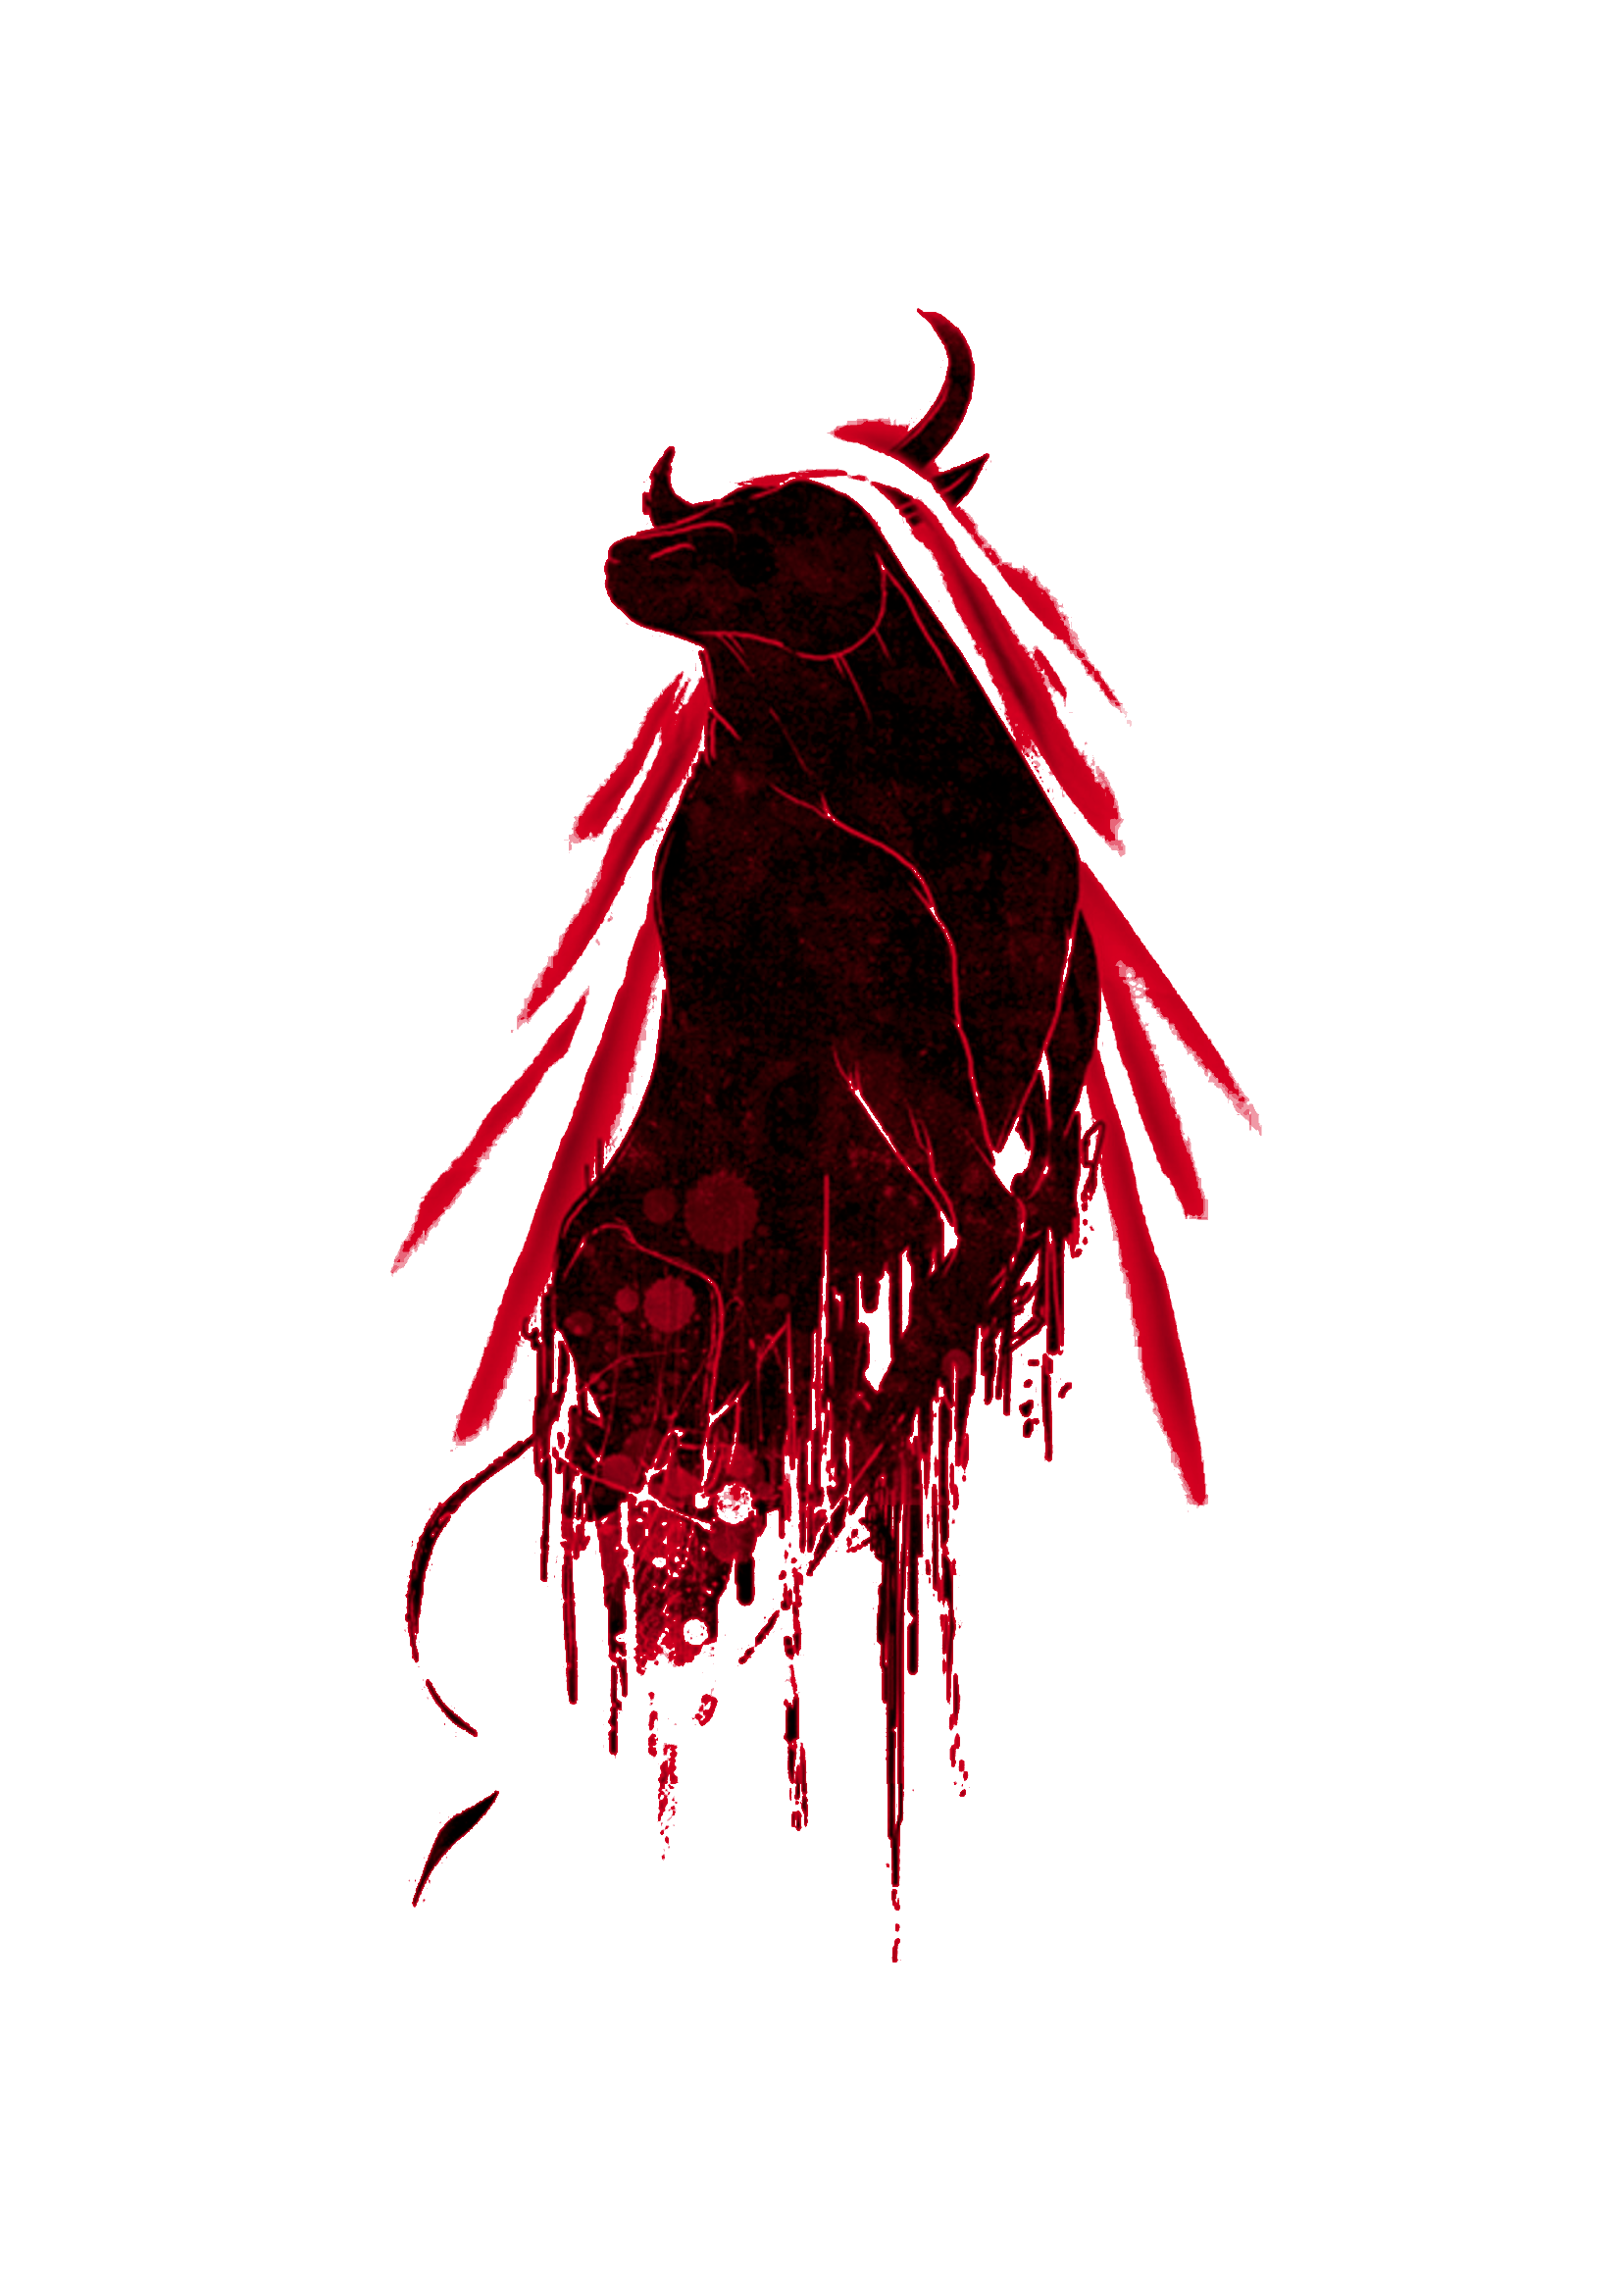
\includegraphics[height=8ex]{logo}}
}
\cfoot{\color{color1}MSR 2018 - Gothenburg, Sweden}
\rfoot{\color{color1}\thepage}
\renewcommand\headrulewidth{0pt}
\renewcommand\footrulewidth{0pt}

%%% picture on cover page
\usepackage{eso-pic}
\newcommand\BackgroundPic{%
\put(0,0){%
\parbox[b][\paperheight]{\paperwidth}{%
\vfill
\centering
\begin{Huge}
{\bf CONFERENCE BOOK} \\
\end{Huge}
\vspace{1cm}

\includegraphics{cover}% 
\vspace{1cm}
\begin{Large}
\\
15\textsuperscript{th} International Conference on Mining Software Repositories \\
Gothenburg, Sweden, May 28\textsuperscript{th}-29\textsuperscript{th} 2018 \\
\end{Large}
\vfill
}}}
%%%
% custom titlepage
\makeatletter
\renewcommand{\maketitle}{
\thispagestyle{empty}
\AddToShipoutPicture*{\BackgroundPic}
\ClearShipoutPicture
%
\phantom{a}
\vfill
\phantom{a}\hfill
\begin{tabular}[c]{@{}p{0.7\textwidth}@{}}
      \color{white}\headingfont\LARGE\@title\\[1em]
      \color{white}\headingfont\Large\@author\\[2em]
\end{tabular}
%
\vspace{0.1cm}
\hspace{12cm} {\tiny https://github.com/gregoriorobles/ConfBookGenerator} \\[0.01em]

\vspace{-1.1cm}
\hspace{12cm} {\tiny (with special thanks to Seila Oliva Muñoz)}
\clearpage
}
\makeatother
%%%


%%% fancy boxes
\usepackage{tcolorbox}
\usepackage{wrapfig}
%\def\namesurname{\color{xº}\headingfont\bfseries\uppercase}{\thesubsubsection}{1em}{}

\def\fullboxbegin{
\bigskip
\begin{tcolorbox}[colback=color1,colframe=color1,coltext=white,arc=0mm,boxrule=0pt]
}
\def\fullboxend{\end{tcolorbox}\medskip}
%
\def\leftboxbegin{
\begin{wrapfigure}{l}{0.5\textwidth}
\begin{tcolorbox}[colback=color1,colframe=color1,coltext=white,arc=0mm,boxrule=0pt]
}
\def\leftboxend{
\end{tcolorbox}
\end{wrapfigure}
}
%
\def\rightboxbegin{
\begin{wrapfigure}{r}{0.5\textwidth}
\begin{tcolorbox}[colback=color1,colframe=color1,coltext=white,arc=0mm,boxrule=0pt]
}
\def\rightboxend{
\end{tcolorbox}
\end{wrapfigure}
}
%
\newcounter{frames}
\def\frameboxbegin#1{
\bigskip
\refstepcounter{frames}
\begin{tcolorbox}[colback=white,colframe=color1,arc=0mm,title={\MakeUppercase{#1}}]
}
\def\frameboxend{
\end{tcolorbox}
}
%%%


\usepackage{lipsum}
\usepackage[spanish]{babel}
\setcounter{page}{0}

%%%%%%%%%%%%%%%
% Title Page
\title{}
\author{}
\date{}
%%%%%%%%%%%%%%%

\begin{document}
\maketitle

%\tableofcontents
\clearpage

\section*{About SATToSE 2017}
SATToSE is the Seminar Series on Advanced Techniques \& Tools for Software Evolution. Its 10th edition takes place in Madrid (Spain) on 7–9 June 2017. Past editions of SATToSE saw presentations on software visualisation techniques, tools for co-evolving various software artefacts, their consistency management, runtime adaptability and context-awareness, as well as empirical results about software evolution.

The goal of SATToSE is to gather both undergraduate and graduate students to showcase their research, exchange ideas, improve their communication skills, attend and contribute technology showdown and hackathons.

This year's SATToSE has a previous, co-located event: the SENECA European project training for PhDs, a one-day seminar on ``writing up \& moving on'' and ``commercializing research'', that will have five renowned speakers. Those who register for SATToSE will have the possibility to attend this event for free.

\section*{Organisation}
\begin{itemize}
 \item General Chair
 \begin{itemize}
  \item \href{https://gsyc.urjc.es/~grex/}{Gregorio Robles}, Universidad Rey Juan Carlos, Spain.
 \end{itemize}
 \item Program Chairs
 \begin{itemize}
  \item \href{http://scg.unibe.ch/staff/osman}{Haidar Osman}, University of Bern, Switzerland.
  \item \href{http://scg.unibe.ch/staff/andreichis}{Andrei Chis}, Feenk GmbH, Switzerland.
 \end{itemize}
 \item Hackathon Chair
 \begin{itemize}
  \item \href{http://www.felienne.com/}{Felienne Hermans}, Delft University of Technology, The Netherlands.
 \end{itemize}
 \item SATToSE Steering Committee
 \begin{itemize}
  \item \href{https://released.info.ucl.ac.be/Members/KimMens}{Kim Mens} (Chair), \href{http://www.ii.uib.no/~anya/}{Anya Helene Bagge}, \href{http://bergel.eu/}{Alexandre Bergel}, \href{https://caracciolo.github.io/}{Andrea Caracciolo}, \href{http://www.inf.usi.ch/phd/dalsat/index.php}{Tommaso Dal Sasso}, \href{http://win.ua.ac.be/~sdemey/}{Serge Demeyer}, \href{http://prog.vub.ac.be/~cderoove}{Coen De Roover}, \href{http://www.di.univaq.it/diruscio/}{Davide Di Ruscio}, \href{http://www.lifl.fr/~etien}{Anne Etien}, \href{http://scg.unibe.ch/staff/Mohammad-Ghafari}{Mohammad Ghafari}, \href{http://plg.uwaterloo.ca/~migod/}{Michael W. Godfrey}, \href{https://sites.google.com/site/andrehoraa/}{André Hora}, \href{https://mircealungu.github.io/}{Mircea Lungu}, \href{http://scg.unibe.ch/staff/Milojkovic}{Nevena Milojković}, \href{http://www.ifi.uzh.ch/en/seal/people/panichella.html}{Sebastiano Panichella}, \href{http://www.inf.usi.ch/phd/ponzanelli/}{Luca Ponzanelli}, \href{http://www.win.tue.nl/~aserebre/}{Alexander Serebrenik}, \href{http://grammarware.net/}{Vadim Zaytsev}
 \end{itemize}
  \item Special thanks to local organizers from the Universidad Rey Juan Carlos
  \begin{itemize}
   \item Jesús Moreno-León, Miguel Ángel Fernández, Gema Rodríguez-Pérez, Dorealda Dalipaj, José Javier Merchante-Picazo, Daniel Izquierdo, Jesús M. González-Barhona, and Alicia Nieto
  \end{itemize}
\end{itemize}

\section*{Participants}

\input{generated}

\end{document}          
